\section{Design and Implementation}
In this section, we introduce the design and implementation details of HydraMini. The structure of the system is shown in Fig.~\ref{fig:framework_overview}. Based on the middle ware, users are able to add more kinds of sensors or create more workers to handle the data while the middle ware provides apis for users to take advantage of computing resource and control the car. It's easy for users to add or remove component to or from the system. 

\begin{figure}[t]
    \centering
    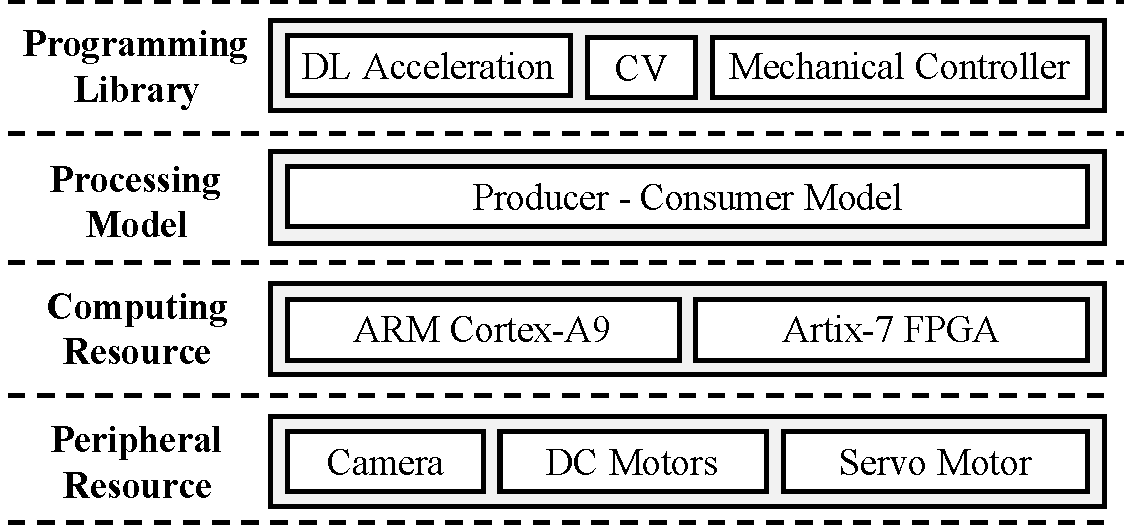
\includegraphics[width=3.25in]{framework_overview}
    \caption{HydraMini Framework Overview.}
    \label{fig:framework_overview}
\end{figure}

\subsection{Hardware Design}
As shown in Fig.~\ref{fig:hardware}, HydraMini is equipped with a Xilinx PYNQ-Z2 board which acts as the main controller, PYNQ\cite{tul2019tulpynqz2} is an open-source project from Xilinx that makes it easy to design embedded systems with Xilinx Zynq Systems on Chips (SoCs). Users create high performance embedded applications with parallel hardware execution, high frame-rate video processing, hardware accelerated algorithms, real-time signal processing, high bandwidth I/O and low latency control. Software developers will take advantage of the capabilities of Zynq and programmable hardware without having to use ASIC-style design tools to design hardware. System architects will have an easy software interface and framework for rapid prototyping and development of their Zynq design. It's suitable to be used in our platform because of the convenience and high performance. The board collects the data from multiple sensors and feeds the data to several computing tasks in real-time. An I/O expansion board V7.1 receives the control message output from the computing tasks and then sends the control signals to the motor drivers to control the movement of HydraMini. The whole HydraMini platform is powered by two Batteries. And to provide steady voltage for PK370PH-4743 motor and DF15MG electric servo motor, a QuicRun WP 1060 Brushed electronic speed controller is used. The basic sensor is one VIMICRO camera, also we provide a study case using LeiShen LS01D LIDAR. It's easy for you to add more sensors to the platform.

\textbf{Programmable Logic (PL)} The programmable logic in PYNQ-Z2 is equivalent to Artix-7 FPGA\cite{2019artix}. The components below are embedded in it:

\begin{itemize}
\item{13,300 logic slices, each with four 6-input LUTs and 8 flip-flops }
\item{630 KB of fast block RAM }
\item{4 clock management tiles, each with a phase locked loop (PLL) and mixed-mode clock manager (MMCM) }
\item{220 DSP slices }
\item{On-chip analog-to-digital converter (XADC) }
\end{itemize}

\textbf{Processing System (PS).} The Cortex-A9\cite{2019arma9} processor is embedded in PYNQ-Z2, it's a performance and power optimized multi-core processor. It features a dual-issue, partially out-of-order pipeline and a flexible system architecture with configurable caches and system coherency using ACP port. The Cortex-A9 processor achieves a better than 50\% performance over the Cortex-A8 processor in a single-core configuration. It has an L1 cache subsystem that provides full virtual memory capabilities. The Cortex-A9 processor implements the ARMv7-A architecture and runs 32-bit ARM instructions, 16-bit and 32-bit Thumb instructions, and 8-bit Java bytecodes in Jazelle state.

\begin{figure}[t]
    \centering
    \includegraphics[width=3.5in]{hardware}
    \caption{HydraMini Hardware Design.}
    \label{fig:hardware}
\end{figure}

\subsection{Software Design}
\textbf{Framework Overview.} The operating system on PYNQ-Z2 is based on Ubuntu 18.04, so libraries are easily installed. The system on PYNQ-Z2 also provides many jupyter notebook documents about how to fully utilize the hardware resources in PYNQ-Z2. To make the control process more efficient and easier to extend, we implement a producer-consumer model\cite{producerconsumer} which is a classic design pattern in multi-process synchronization environment. The whole control system depends on three main components: mechanical controller, AI model inference and computer vision analysis. 

\textbf{Producer-Consumer model.} Many indoor AD driving platforms like HydraOne\cite{wang2019hydraone} and F1/10\cite{o2019f1} use ROS\cite{quigley2009ros} to manage the hardware and software resources nowadays because ROS provides the car with an easy way to communicate with the server and many existing applications. However, to make a balance between the platform's cost and performance, we focuses mainly on core functions in AD and the communication between car and server is not so important. Using ROS will bring unnecessary overhead to CPU. So a more streamlined and efficient method is used as the base of the control system. Refer to Fig.~\ref{fig:producer_consumer} for an overview of this model.

\begin{figure}[t]
    \centering
    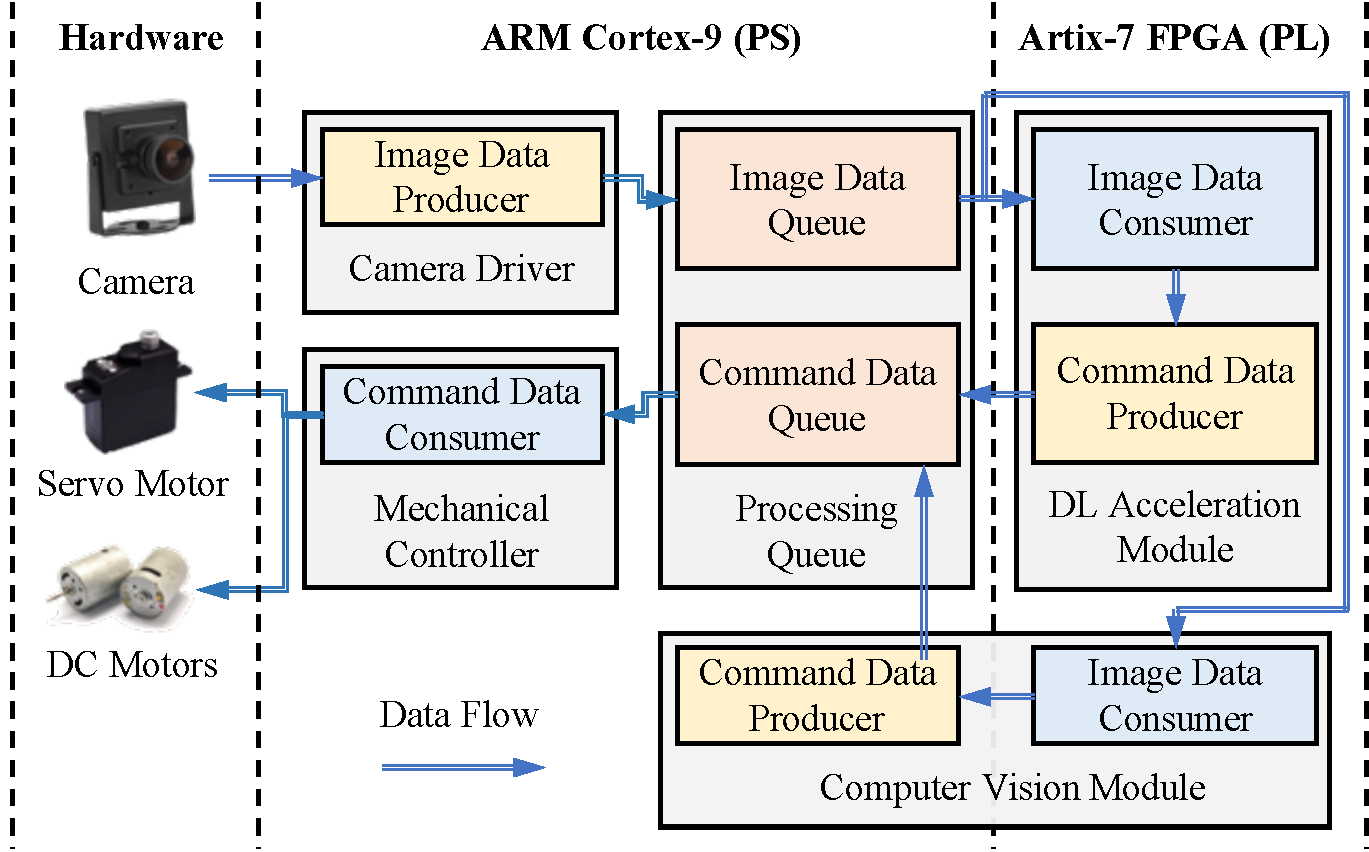
\includegraphics[width=3.25in]{producer_consumer}
    \caption{Producer-Consumer Model.}
    \label{fig:producer_consumer}
\end{figure}

The sensors like camera will play the role of producer while the decision makers like AI model and computer vision methods will be consumers. Each kind of data will be stored in a queue in memory. Different producer processes add the data they get to the specified queue and will be handled by consumers who cares about this kind of data. It's easy to add more producers or consumers and new kind of data. If one process want to handle or provide different kind of data, just read or write the related queue. The synchronism of the system is maintained by locks, each queue will have a lock.

The consumers who usually act as controller have a shared clock. They will check if their commands to send is outdated according to the clock, this clock ensures that the car won't receive outdated commands. Also, there exists a token which indicates who has the current property in control power. Users are able to define their own strategy for the transformation of property.

\textbf{Mechanical Controller.} The HydraMini platform has one motor for providing power and one servo motor for direction control. This design has been widely used in real cars. We provide basic control apis for users. The rotate speed of the motor and the angle of deflection of servo motor are set directly. Also higher level methods like accelerating are provided too. 

Besides driving on its own, the car is controlled by using the keyboard. We invoke OpenCV\cite{opencv} library to read the keyboard signals and then call the mechanical api. Users are able to define their own button layout easily. This ability is mostly used to generate training data.

\textbf{AI Inference.} AI technology is an important part in AD, it handles many tasks like objects identification, lane keeping and so on. In our platform AI inference process is packed as a consumer thread, it reads data from produced data queue and use it as the input of AI network. Then the model produces control commands directly or just provide information for controller thread to make decisions. 

And with the power of DPU\cite{dnndk} which is one accelerator in FPGA, the process of AI reference will be accelerated. The AI inference thread is copied and they run concurrently in DPU, which means higher inference performance. 

To make good use of DPU and to make the optimization process easy, we provide scripts to do a complete set of optimized tool chains provided by DNNDK, including compression, compilation and runtime. Refer to Fig.~\ref{fig:dnndk} to see the framework of DNNDK. First the Deep Compression Tool DECENT\cite{dnndk}, employs coarse-grained pruning, trained quantization and weight sharing to make the inference process in edge meet the low latency and high throughput requirement with very small accuracy degradation. Second the DNNC (Deep Neural Network Compiler)\cite{dnndk} which is the dedicated proprietary compiler designed for the DPU will map the neural network algorithm to the DPU instructions to achieve maxim utilization of DPU resources by balancing computing workload and memory access. Third the users use the Cube of Neutral Networks (N2Cube)\cite{dnndk} the DPU runtime engine to load DNNDK applications and manage resource allocation and DPU scheduling. Its core components include DPU driver, DPU loader, tracer, and programming APIs for application development.

After using DPU, the performance of end-to-end model described in case study is up to $7,000$ FPS which is fast enough to satisfy the requirement of low-latency in AD. We also test YoloV3\cite{redmon2018yolov3} model in DPU and it achieves 3 fps when detecting 80 categories of things.

\begin{figure}[t]
    \centering
    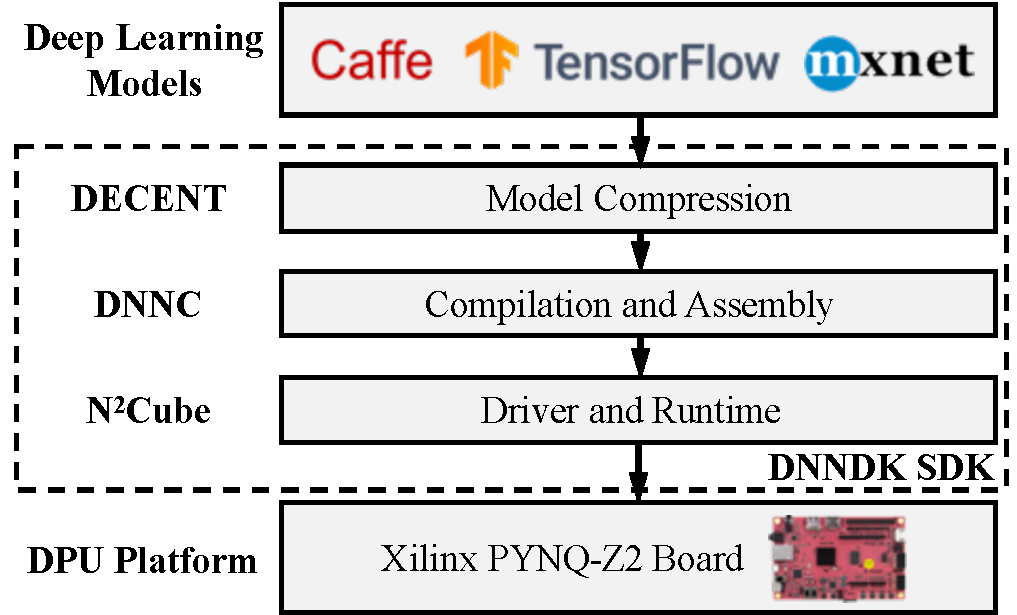
\includegraphics[width=3.25in]{dnndk.pdf}
    \caption{DNNDK Framework.}
    \label{fig:dnndk}
\end{figure}

\textbf{Computer Vision Analysis.} OpenCV\cite{opencv} is a widely used library for computer vision analysis. Due to the native support for OpenCV in PYNQ-Z2, existing computer vision algorithms are easily invoked and their own algorithms can be implemented. We have a case below which shows how to use traditional computer vision methods to manage AD tasks. The control process of these methods is just the same as AI model's, the thread running computer vision algorithms will read data from producers and output commands or information. More threads can be created to increase throughput. 

However, these computer vision algorithms may be very time consuming running in ARM Cortex-A9 in Xilinx PYNQ-Z2. To reduce computation complexity, we do several pre-process like cropping and down-sampling. Time consuming tasks such as Gaussian filter, Canny edge detection, Hough transform can be moved to FPGA using Xilinx xfopencv library\cite{xfopencv}, BP neural network can be implemented in FPGA using Xilinx Vivado HLS. However, when implementing accelerators in FPGA, users should take the board's resource into consideration and choose the heaviest computational task to implement while not beyond the resource limit. If there remains enough PL space for your algorithms, you put them in PL side, or just put them in PS side.